\section{Auswertung}

In der folgenden Auswertung werden alle Berechnungen mit Python durchgeführt.
Bei der linearen Regression wird an eine Funktion der folgenden Form gefittet:

\begin{equation}
  \label{eqn:Regression0}
  f(\su{x}) = \su{m} \cdot \su{x} + \su{b}
\end{equation}


\subsection{Bestimmung der Gegenspannung für die verschiedenen Spektralfarben}

Für die Bestimmung der Gegenspannung der gelben Spektrallinie werden aus der Tabelle
9 lediglich die Werte für $U$ $\geq \SI{0}{\volt}$ betrachtet und in
Abb. \ref{fig:Gelb} grafisch dargestellt.

Mithilfe einer linearen Regression gemäß der Formel \eqref{eqn:Regression0} wird die
Gegenspannung bestimmt, indem der Schnittpunkt der Ausgleichsgeraden mit der
Spannungsachse nach folgender Formel ermittelt wird:

\begin{equation}
  \su{x}\ua{0} = - \frac{\su{b}}{\su{m}}.
\end{equation}

Damit ergeben sich für die Gegenspannungen der verschiedenen Spektralfarben
die folgenden Werte.

\begin{table}
  \centering
  \label{tab:Spannungen}
  \caption{Bestimmte Grenzspannungen für verschiedene Spektralfarben.}
  \begin{tabular}{c c c}
    \toprule
    $\lambda$ in $\si{nm}$ & $U\ua{g}$ in $\si{V}$ & $\sigma\ua{U}$ in $\si{V}$ \\
    \midrule
    578 & 0.56 & 0.03\\
    546 & 0.67 & 0.04 \\
    492 & 0.86 & 0.03 \\
    435 & 1.13 & 0.06 \\
    405 & 1.17 & 0.05 \\
    365 & 1.15 & 0.08 \\
    \bottomrule
  \end{tabular}
\end{table}


Die für die Bestimmung der Gegenspannung verwendeten Parameter aus der linearen
Regression für die einzelnen Farbspektren sind noch einmal in Tabelle
\ref{tab:Messparameter} zu sehen.

Im Folgenden sind die gemessenen Messwerte sowie die dazugehörigen
Abbildungen für jede Spektralfarbe zu sehen. Die Abweichungen von den gemessenen und
errechneten Nullstellen kommen vermutlich daher, dass bei den gemessenen Nullstellen
schon ein negativer Photostrom vorhanden war, welcher allerdings nicht angezeigt
wurde.

\newpage

\begin{table}
  \centering
  \label{tab:Gelb}
  \caption{Aufgenommene Werte bei der gelben Spektralfarbe.}
  \begin{tabular}{c c c }
    \toprule
    $U$ in $\su{V}$ & $I\cdot 10^{9}$ in $\su{A}$ & $\sqrt{I}\cdot10^{5}$ in $\su{A}^{\frac{1}{2}}$ \\
    \midrule
     0     & 0.7  & 2.65 \\
     0.1   & 0.45 & 2.12 \\
     0.2   & 0.32 & 1.79 \\
     0.31  & 0.14 & 1.18 \\
     0.4   & 0.05 & 0.7  \\
     0.55  & 0    & 0    \\
     \bottomrule
   \end{tabular}
 \end{table}


\begin{figure}
  \centering
  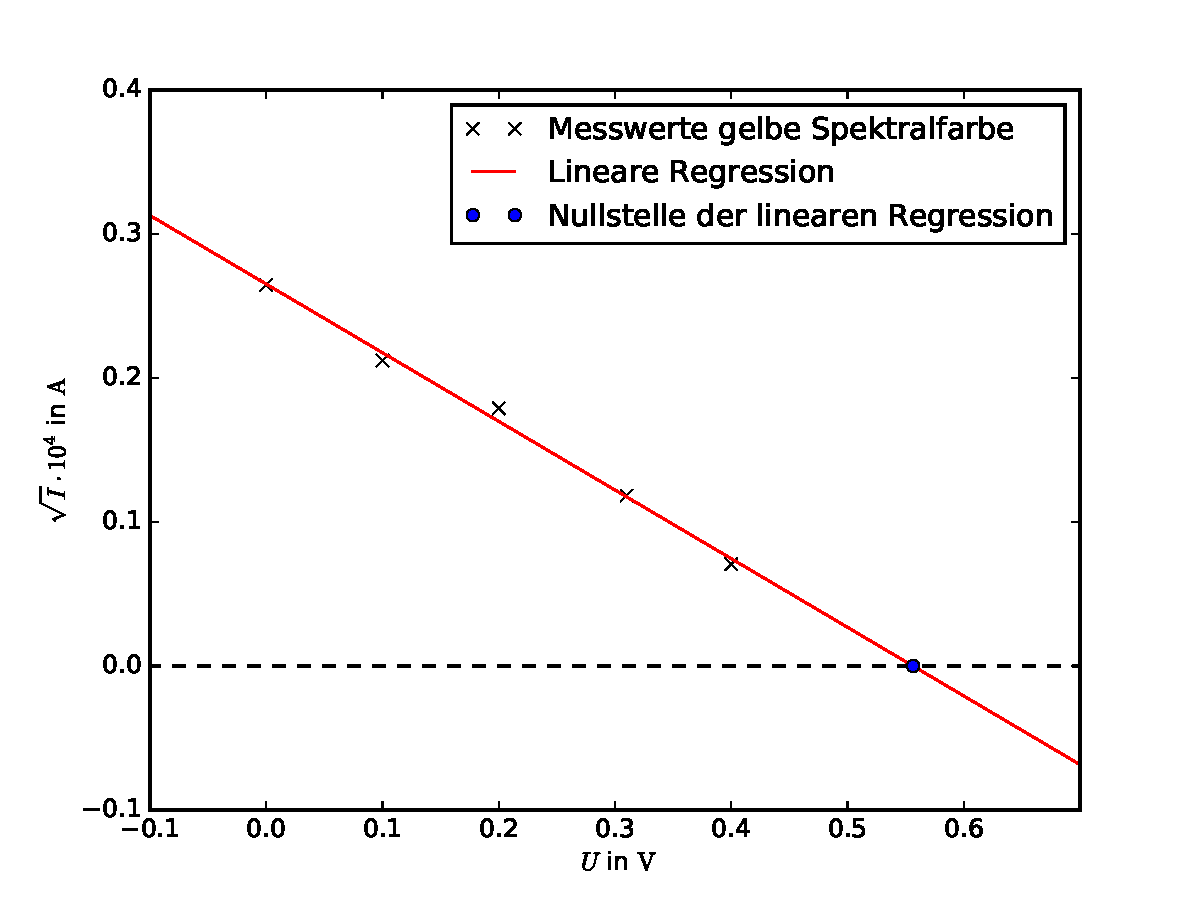
\includegraphics[width = 0.8\textwidth]{Pics/gelbe_Spektrallinie.pdf} \\[0cm]
  \caption{Gemessene Stromstärke in Abhängigkeit der angelegten Spannung für die
           gelbe Spektralfarbe.}
  \label{fig:Gelb}
\end{figure}

\newpage


\begin{table}
  \centering
  \label{tab:Gelb_Komplett}
  \caption{Aufgenommene Werte bei der gruenen Spektralfarbe.}
  \begin{tabular}{c c c}
    \toprule
    $U$ in $\su{V}$ & $I\cdot 10^{9}$ in $\su{A}$ & $\sqrt{I}\cdot10^{5}$ in $\su{A}^{\frac{1}{2}}$ \\
    \midrule
    0.01 & 1.2  & 3.46 \\
    0.1  & 1    & 3.16 \\
    0.2  & 0.8  & 2.83 \\
    0.3  & 0.5  & 2.24 \\
    0.4  & 0.22 & 1.48 \\
    0.5  & 0.09 & 0.95 \\
    0.6  & 0.02 & 0.45 \\
    0.64 & 0    & 0    \\
    \bottomrule
  \end{tabular}
\end{table}


\begin{figure}
  \centering
  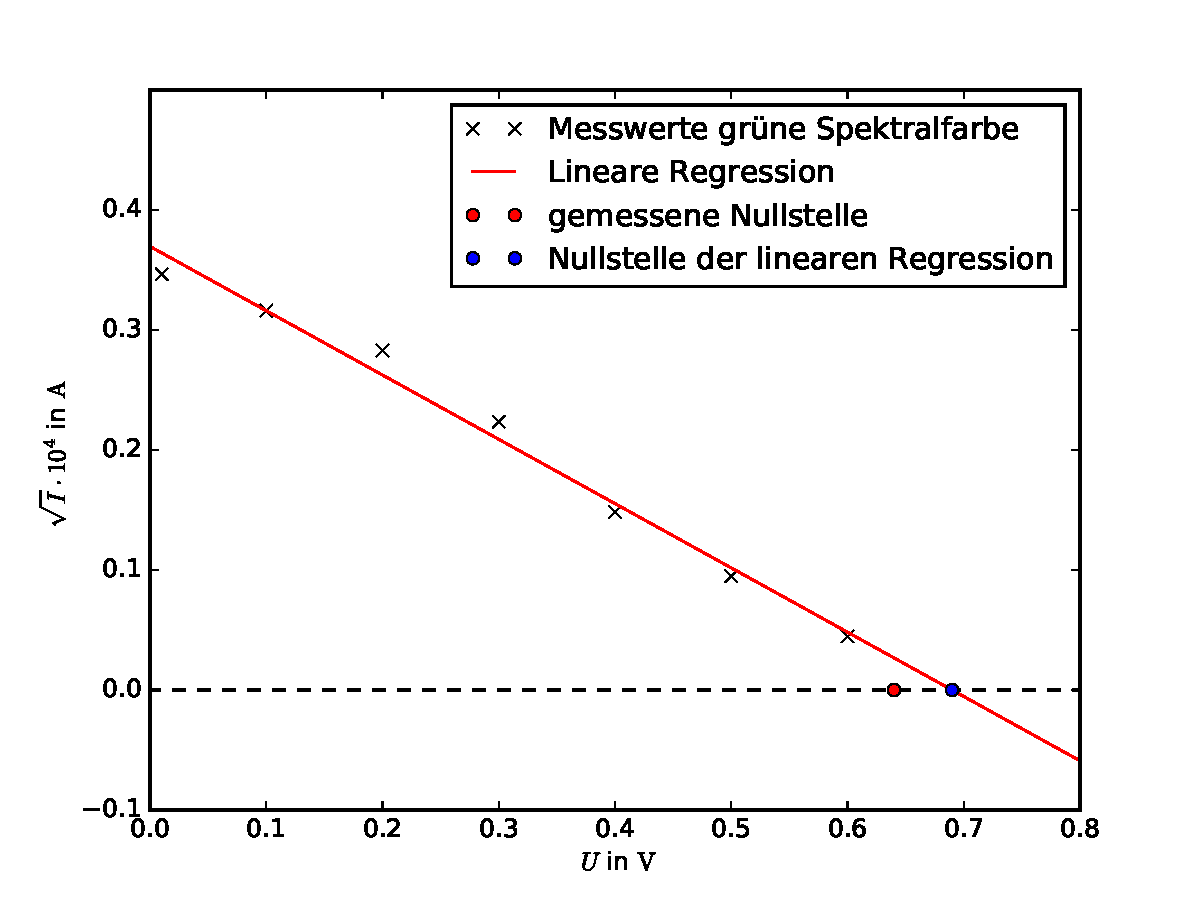
\includegraphics[width = 0.7\textwidth]{Pics/gruene_Spektrallinie.pdf}\\[0cm]
  \caption{Gemessene Stromstärke in Abhängigkeit der angelegten Spannung für die
           grüne Spektralfarbe.}
  \label{fig:Gruen}
\end{figure}

\newpage

\begin{table}
  \centering
  \label{tab:blaugruen}
  \caption{Aufgenommene Werte bei der blau-grünen Spektralfarbe.}
  \begin{tabular}{c c c | c c c}
    \toprule
    $U$ in $\su{V}$ & $I\cdot 10^{9}$ in $\su{A}$ & $\sqrt{I}\cdot10^{5}$ in $\su{A}^{\frac{1}{2}}$ &
    $U$ in $\su{V}$ & $I\cdot 10^{9}$ in $\su{A}$ & $\sqrt{I}\cdot10^{5}$ in $\su{A}^{\frac{1}{2}}$ \\
    \midrule
    0.01  & 0.3  & 1.73 & 0.45  & 0.08 & 0.89 \\
    0.05  & 0.29 & 1.7  & 0.55  & 0.04 & 0.63 \\
    0.1   & 0.22 & 1.48 & 0.6   & 0.03 & 0.55 \\
    0.151 & 0.2  & 1.41 & 0.65  & 0.02 & 0.45 \\
    0.202 & 0.2  & 1.41 & 0.7   & 0.01 & 0.32 \\
    0.253 & 0.18 & 1.34 & 0.75  & 0.01 & 0.32 \\
    0.3   & 0.15 & 1.22 & 0.8   & 0    & 0    \\
    0.35  & 0.12 & 1.1  &       &      &      \\
    \bottomrule
  \end{tabular}
\end{table}


\begin{figure}
  \centering
  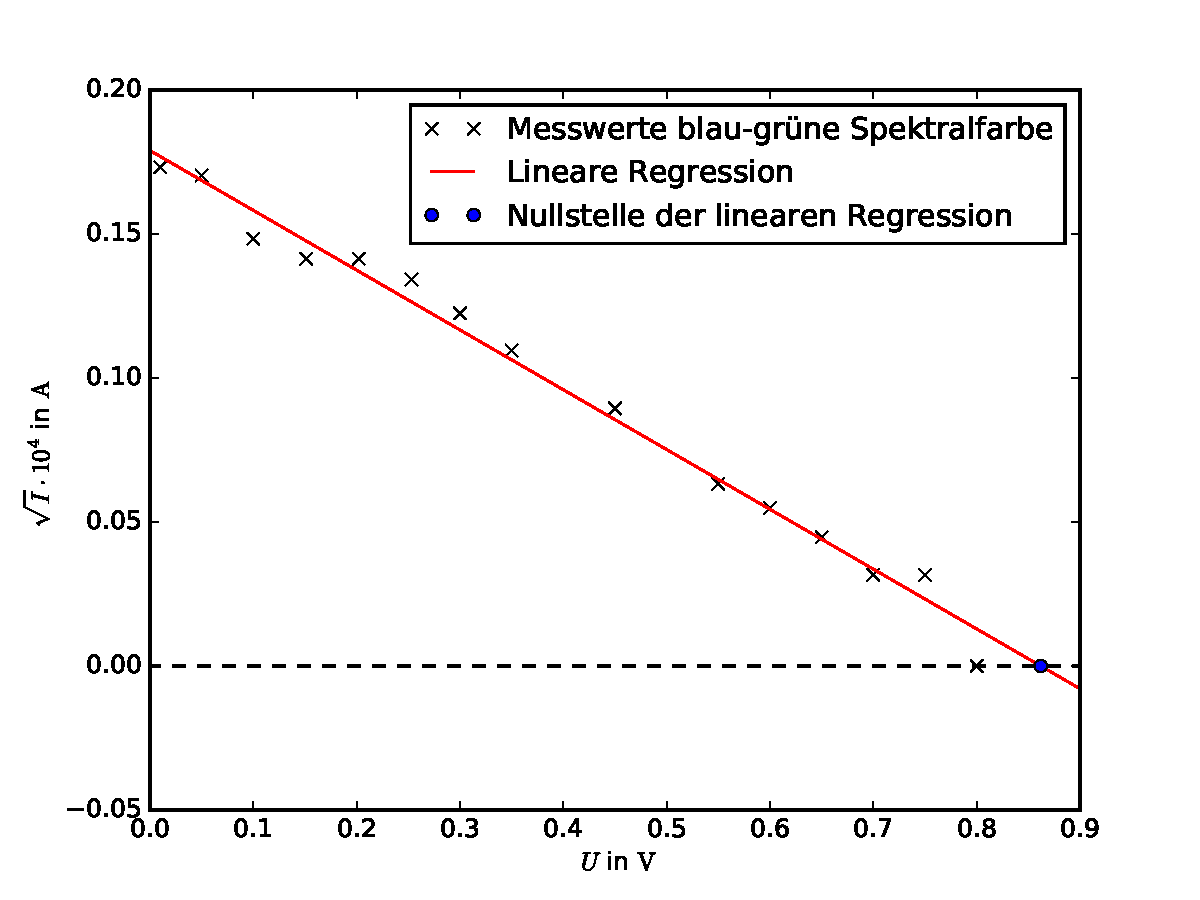
\includegraphics[width = 0.7\textwidth]{Pics/blau_gruene_Spektrallinie.pdf}\\[0cm]
  \caption{Gemessene Stromstärke in Abhängigkeit der angelegten Spannung für die
           blau-grüne Spektralfarbe.}
  \label{fig:BlauGruen}
\end{figure}

\newpage

\begin{table}
  \centering
  \label{tab:blau}
  \caption{Aufgenommene Werte bei der blauen Spektralfarbe.}
  \begin{tabular}{c c c | c c c}
    \toprule
    $U$ in $\su{V}$ & $I\cdot 10^{9}$ in $\su{A}$ & $\sqrt{I}\cdot10^{5}$ in $\su{A}^{\frac{1}{2}}$ &
    $U$ in $\su{V}$ & $I\cdot 10^{9}$ in $\su{A}$ & $\sqrt{I}\cdot10^{5}$ in $\su{A}^{\frac{1}{2}}$ \\
    \midrule
    0.01 & 7.4  & 8.6  & 0.6  & 2.3  & 4.8  \\
    0.1  & 6.6  & 8.12 & 0.7  & 1.4  & 3.74 \\
    0.21 & 6.4  & 8    & 0.81 & 0.6  & 2.45 \\
    0.31 & 5.6  & 7.48 & 0.9  & 0.33 & 1.82 \\
    0.4  & 4.0  & 6.32 & 1.0  & 0.1  & 1    \\
    0.5  & 3.2  & 5.66 & 1.07 & 0    & 0    \\
    \bottomrule
  \end{tabular}
\end{table}


\begin{figure}
  \centering
  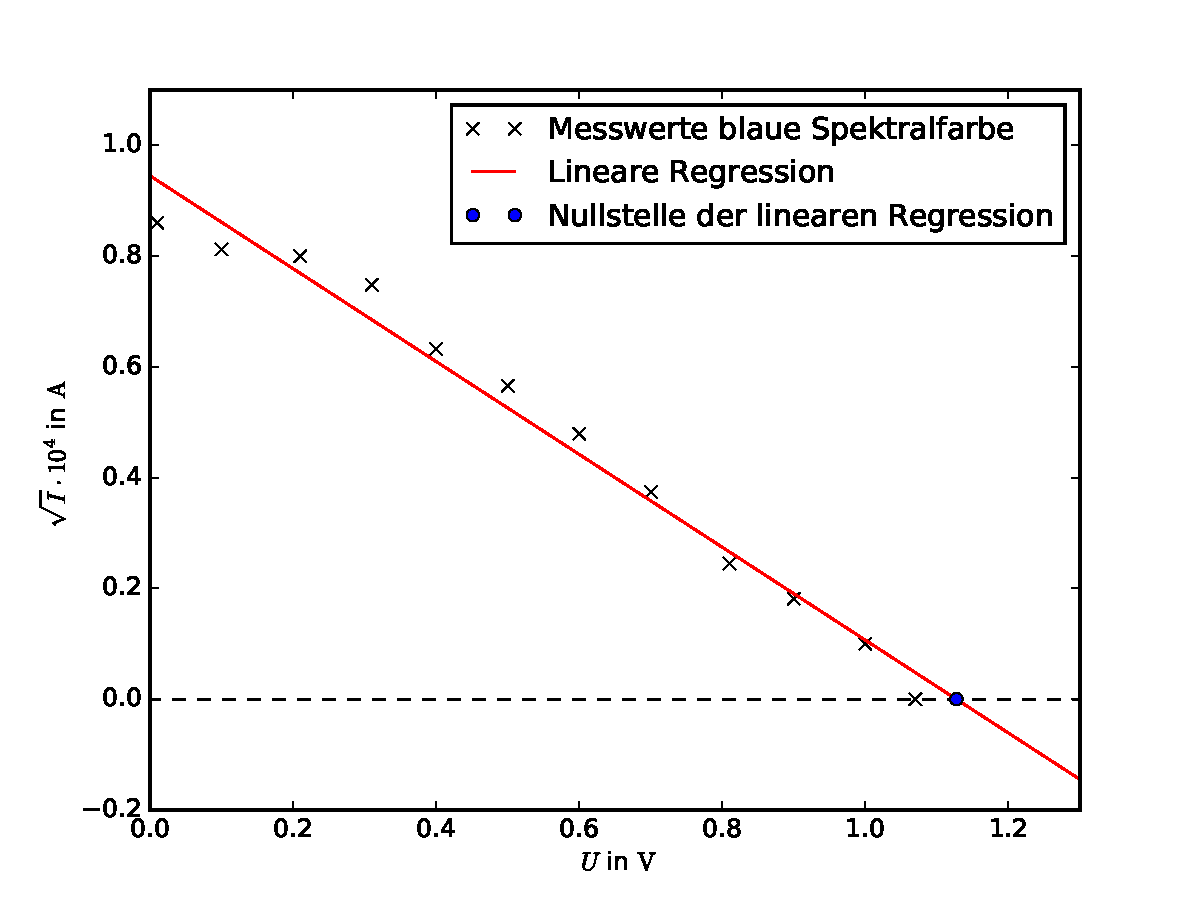
\includegraphics[width = 0.8\textwidth]{Pics/blaue_Spektrallinie.pdf}\\[0cm]
  \caption{Gemessene Stromstärke in Abhängigkeit der angelegten Spannung für die
           blaue Spektralfarbe.}
  \label{fig:Blau}
\end{figure}

\newpage

\begin{table}
  \centering
  \label{tab:UV1}
  \caption{Aufgenommene Werte bei der 1. ultravioletten Spektralfarbe.}
  \begin{tabular}{c c c | c c c}
    \toprule
    $U$ in $\su{V}$ & $I\cdot 10^{9}$ in $\su{A}$ & $\sqrt{I}\cdot10^{5}$ in $\su{A}^{\frac{1}{2}}$ &
    $U$ in $\su{V}$ & $I\cdot 10^{9}$ in $\su{A}$ & $\sqrt{I}\cdot10^{5}$ in $\su{A}^{\frac{1}{2}}$ \\
    \midrule
    0.001 & 2.7  & 5.2  & 0.7   & 0.52 & 2.28 \\
    0.1   & 2.4  & 4.9  & 0.8   & 0.28 & 1.67 \\
    0.2   & 2.2  & 4.7  & 0.9   & 0.16 & 1.26 \\
    0.3   & 1.9  & 4.36 & 1     & 0.08 & 0.89 \\
    0.4   & 1.7  & 4.12 & 1.1   & 0.01 & 0.32 \\
    0.5   & 1.1  & 3.32 & 1.12  & 0    & 0    \\
    0.6   & 0.7  & 2.65 & 0     &      &      \\
    \bottomrule
  \end{tabular}
\end{table}


\begin{figure}
  \centering
  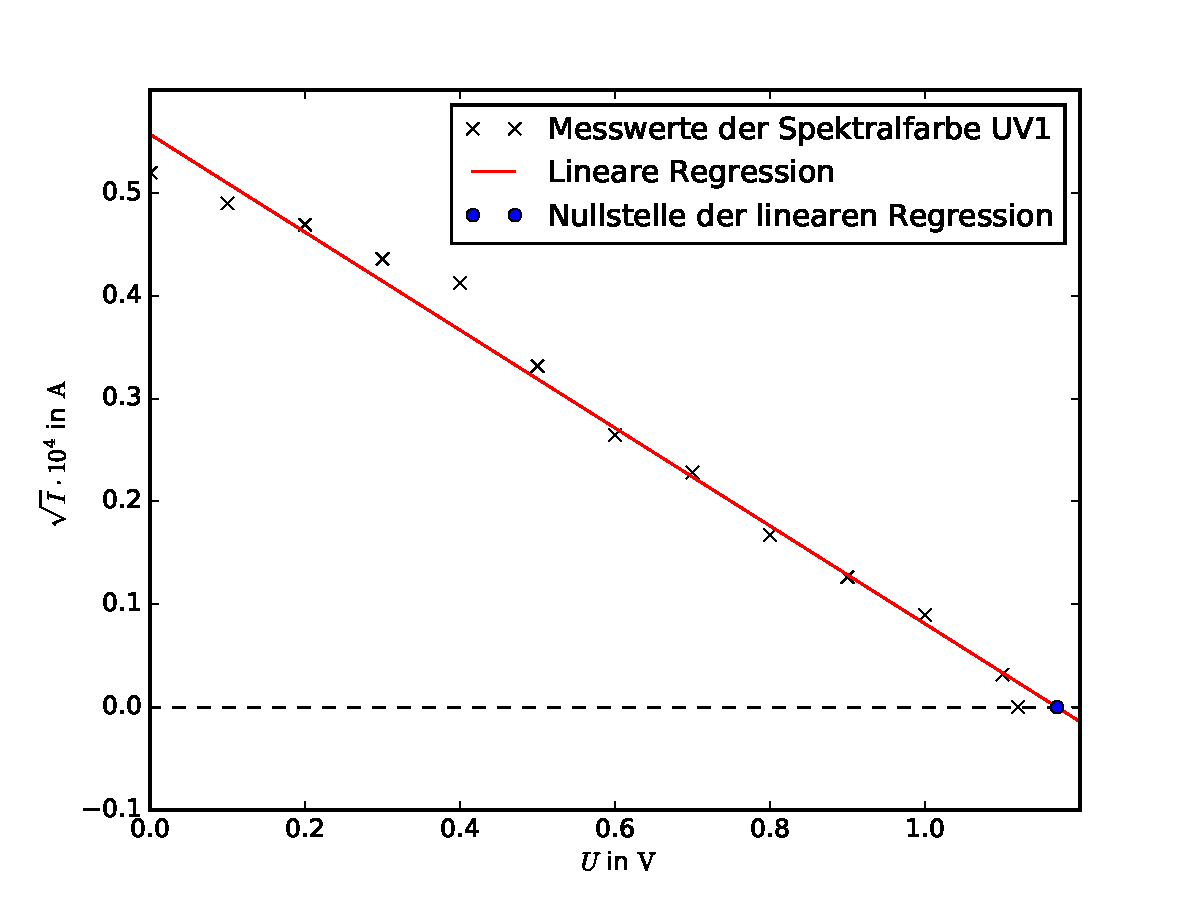
\includegraphics[width = 0.75\textwidth]{Pics/UV1_Spektrallinie.pdf}\\[0cm]
  \caption{Gemessene Stromstärke in Abhängigkeit der angelegten Spannung für die
           1. ultraviolette Spektralfarbe.}
  \label{fig:UV1}
\end{figure}

\newpage

\begin{table}
  \centering
  \label{tab:Gelb_Komplett}
  \caption{Aufgenommene Werte bei der 2. ultravioletten Spektralfarbe.}
  \begin{tabular}{c c c}
    \toprule
    $U$ in $\su{V}$ & $I\cdot 10^{9}$ in $\su{A}$ & $\sqrt{I}\cdot10^{5}$ in $\su{A}^{\frac{1}{2}}$ \\
    \midrule
    0.001 & 0.3  & 1.73 \\
    0.1   & 0.26 & 1.61 \\
    0.2   & 0.23 & 1.52 \\
    0.3   & 0.19 & 1.38 \\
    0.4   & 0.16 & 1.26 \\
    0.5   & 0.12 & 1.1  \\
    0.6   & 0.09 & 0.95 \\
    0.7   & 0.06 & 0.77 \\
    0.8   & 0.04 & 0.63 \\
    0.9   & 0.02 & 0.45 \\
    1     & 0    & 0    \\
    \bottomrule
  \end{tabular}
\end{table}


\begin{figure}
  \centering
  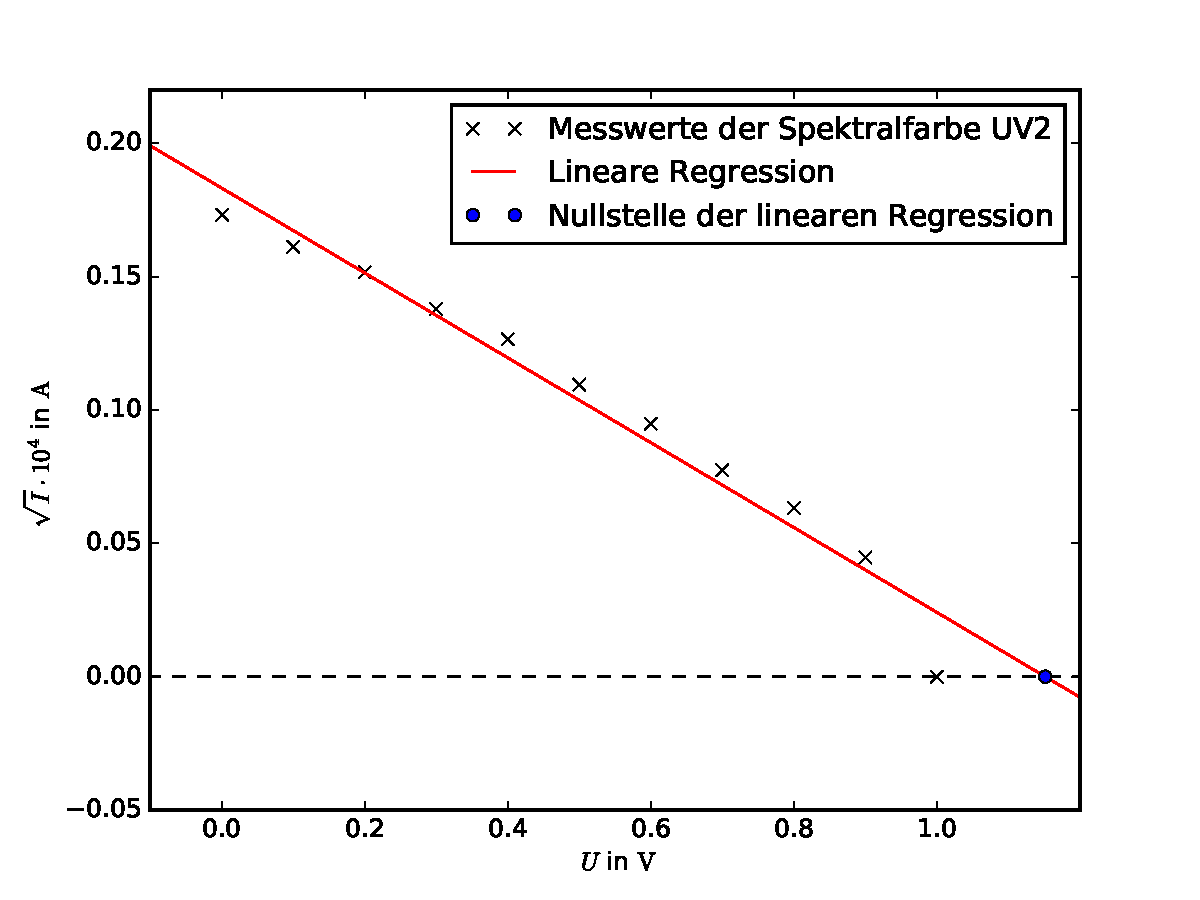
\includegraphics[width = 0.75\textwidth]{Pics/UV2_Spektrallinie.pdf}\\[0cm]
  \caption{Gemessene Stromstärke in Abhängigkeit der angelegten Spannung für die
           2.ultraviolette Spektralfarbe.}
  \label{fig:UV2}
\end{figure}

\newpage

Die folgenden Parameter für Steigung und Achsenabschnitt wurden aus der linearen
Regression gemäß Formel \eqref{eqn:Regression0} entnommen. Die angegebenen Fehler
wurden dabei mit Python berechnet.

\begin{table}
  \centering
  \caption{Bestimmte Werte für die Steigung sowie den Achsenabschnitt der
           linearen Regression für die verschiedenen Farbspektren.}
  \label{tab:Messparameter}
  \begin{tabular}{c | c c}
    \toprule
    Farbspektrum & (m $\pm$ $\increment$m) $\cdot 10^5$ in $\frac{\su{A}^{\sfrac{1}{2}}}{\su{V}}$ &
    (b $\pm$ $\increment$b) $\cdot 10^5$ in $\su{A}^{\sfrac{1}{2}}$ \\
    \midrule
    Gelb      & -4.59 $\pm$ -0.29 & 2.63 $\pm$ 0.06 \\
    Grün      & -5.36 $\pm$ -0.28 & 3.70 $\pm$ 0.10 \\
    Blau      & -8.10 $\pm$ -0.40 & 9.37 $\pm$ 0.24 \\
    Blau-Grün & -2.01 $\pm$ -0.06 & 1.77 $\pm$ 0.03 \\
    UV1       & -4.66 $\pm$ -0.18 & 5.54 $\pm$ 0.12 \\
    UV2       & -1.43 $\pm$ -0.04 & 1.78 $\pm$ 0.02 \\
    \bottomrule
  \end{tabular}
\end{table}


\newpage
\newpage

\subsection{Bestimmung der Austrittsarbeit $A\ua{k}$ und des Verhältnisses $\frac{h}{e\ua{0}}$}

\begin{align}
  U\ua{g}   &= \frac{h}{e\ua{0}} \cdot \nu + \frac{A\ua{k}}{e\ua{0}}
  \label{eqn:Regression1} \\
  f(\su{x}) &= \su{m} \cdot \su{x} + \su{b}
  \label{eqn:Regression2} \\
  \su{m}  &= \frac{h}{e\ua{0}}
  \label{eqn:Regression3} \\
  \su{b}  &= \frac{A\ua{k}}{e\ua{0}}.
  \label{eqn:Regression4}
\end{align}

\begin{figure}
  \centering
  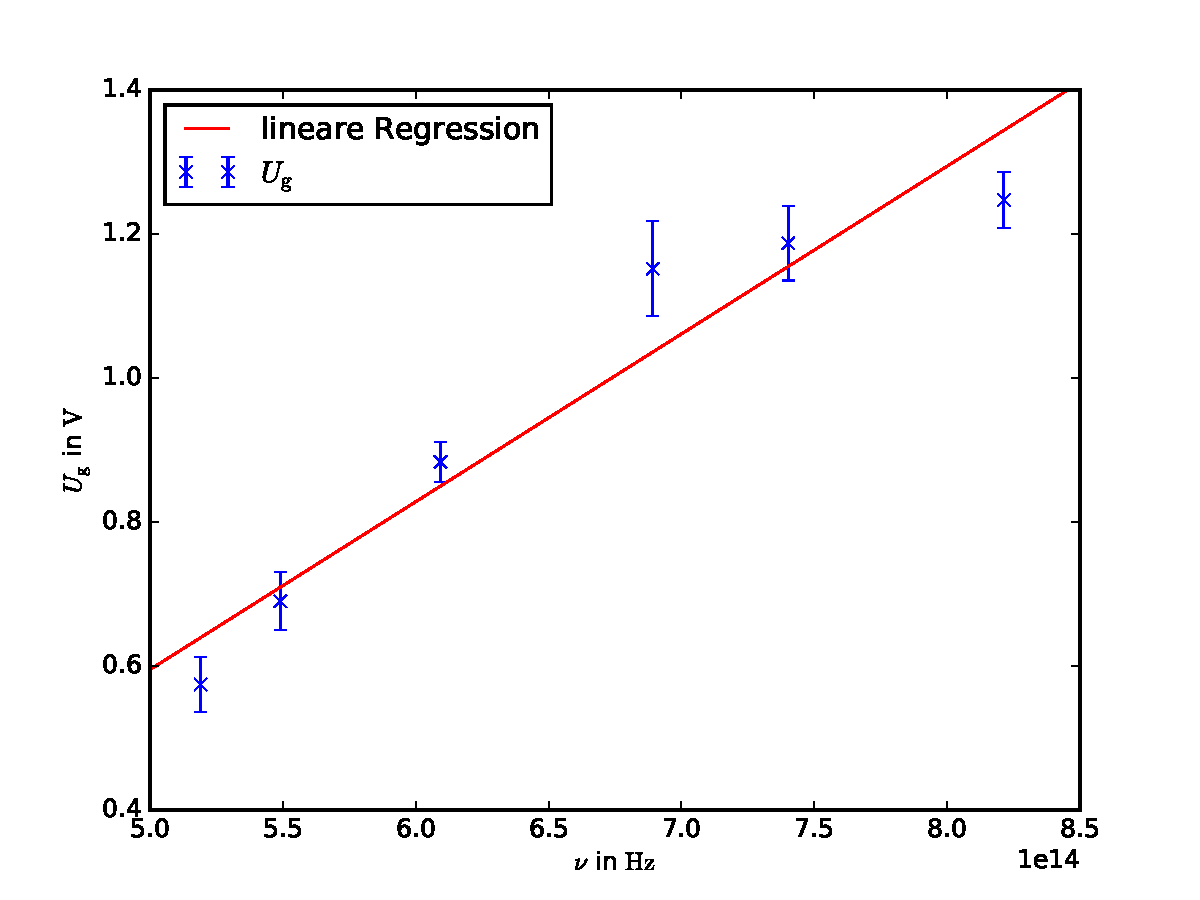
\includegraphics[width = 0.8\textwidth]{Pics/U_g_gegen_Frequenz.pdf}
  \caption{Gegenspannungen der verschiedenen Lichtfrequenzen.}
  \label{fig:Gegenspannung}
\end{figure}

Mithilfe der in Messung 3.1 erhaltenen Gegenspannungen für die verschiedenen
Spektralfarben (siehe Tab. 1) lassen sich die gesuchten
Parameter
aus Gleichung \eqref{eqn:Regression1} bestimmen. Dafür wird eine lineare Regression
nach Formel \eqref{eqn:Regression2} durchgeführt (siehe Abb. \ref{fig:Gegenspannung}),
welche für die Parameter folgende Werte ausgibt:

\begin{align}
  m = \frac{h}{e\ua{0}}                 &= \num{2.33(33)e-15} \, \si{eV}\\
  b = \frac{A\ua{k}}{e\ua{0}} = A\ua{k} &= (\num{0.57(22)}) \, \si{eV}
\end{align}

\newpage

\subsection{Betrachtung der gelben Spektralfarbe in einem Intervall von $U \, \in$ $[-20, 20] \, \su{V}$ }

\begin{table}
  \centering
  \label{tab:GelbKomplett}
  \caption{Aufgenommene Werte bei der gelben Spektralfarbe.}
  \begin{tabular}{c c c | c c c }
    \toprule
    $U$ in $\su{V}$ & $I\cdot 10^{9}$ in $\su{A}$ & $\sqrt{I}\cdot10^{5}$ in $\su{A}^{\frac{1}{2}}$ &
    $U$ in $\su{V}$ & $I\cdot 10^{9}$ in $\su{A}$ & $\sqrt{I}\cdot10^{5}$ in $\su{A}^{\frac{1}{2}}$ \\
    \midrule
    -19.15 & 8.3  & 9.11 & -4.04  & 4.3  & 6.56 \\
    -17.05 & 8    & 8.94 & -3.05  & 3.9  & 6.25 \\
    -15.01 & 7.65 & 8.75 & -2.02  & 2.7  & 5.2  \\
    -13.02 & 7.3  & 8.54 & -1.01  & 2    & 4.47 \\
    -10.99 & 6.6  & 8.12 &  0     & 0.7  & 2.65 \\
    -9.99  & 6.4  & 8    &  0.1   & 0.45 & 2.12 \\
    -9.0   & 6.15 & 7.84 &  0.2   & 0.32 & 1.79 \\
    -8.05  & 5.9  & 7.68 &  0.31  & 0.14 & 1.18 \\
    -7.05  & 5.5  & 7.42 &  0.4   & 0.05 & 0.7  \\
    -6.02  & 5.1  & 7.14 &  0.55  & 0    & 0    \\
    -5.05  & 4.8  & 6.93 &        &      &      \\
     \bottomrule
   \end{tabular}
 \end{table}


In dem letzten Teil des Versuches wird noch einmal der Photostrom für die
gelbe Spektralfarbe in einem Messintervall von -20 < U < 5 $\su{V}$ betrachtet.
Die verwendeten Werte sind in die obige Tabelle 9 eingetragen.
Die Abbildung \ref{fig:Komplett1} zeigt das ganze Messintervall und
Abbildung \ref{fig:Komplett2} ein Intervall für -3 < U < 1 $\su{V}$.

Bei Betrachtung der beiden Abbildungen fallen einige Besonderheiten auf. Zum Beispiel
konvergiert die Kurve bei hohen Beschleunigungssannungen gegen einen bestimmten
Grenzwert. Dies wird durch die Eigenschaft hervorgerufen, dass die Anzahl der ausgelösten Elektronen
lediglich von der Lichtintensität abhängt. Bei einer bestimmten Spannung wird somit
die maximale Anzahl an auslösbaren Elektronen erreicht, welche durch eine konstante
Lichtintensität nicht erhöht werden kann.

Dieser Sättigungswert wird allerdings
lediglich asymptotisch errreicht, da auch die Elektronen einer gewissen Streuung
unterliegen. Um dieses Problem auszugleichen, würde eine kugelförmige
Kathode in deren Inneren die Anode von dem Licht bestrahlt wird, benötigt werden.
Solch ein Aufbau würde keinen Elektronenverlust zulassen.

Eine weitere Auffälligkeit ist das Absinken des Photostroms schon vor Erreichen
der Gegenspannung. Dieses Verhalten kann mit der Fermi-Dirac-Verteilung erklärt
werden, da jedes ausgelöste Elektron eine andere Energie besitzt.

Ein bei uns nicht aufgetretener Effekt, aber zur Vollständigkeit im Folgenden
erwähnt, wäre außerdem noch das Auftreten eines dem
Photostrom entegegengerichteten Stromes gewesen.
Dies ist dadurch zu erklären, dass auch die Anode einem lichtelektrischen
Effekt unterworfen ist, der allerdings aufgrund der Oberfläche und des verwendeten
Materials (höhere Bindungsenergie) deutlich geringer ist als bei der Kathode.
Allerdings verdampft das für die Kathode verwendete Material schon bei sehr
geringen Temperaturen. Dadurch könnten sich Materialreste auf der Anode ablagern,
die für eine Verringerung der Austrittsarbeit sorgen.

Jedoch ist die Fläche der
Anode im Vergleich zur Kathode sehr gering und somit wird der Sättigungswert deutlich
schneller erreicht. Tritt der negative Strom schon bei sehr energiearmen Licht auf
(laut Anleitung bei $\lambda\approx\SI{650}{\nano\meter}$, \cite{anleitung01}), ist
die Austrittsarbeit vermutlich ziemlich gering und in der Größenordnung der Kathode.


\begin{figure}
  \centering
  \begin{subfigure}{0.8\textwidth}
    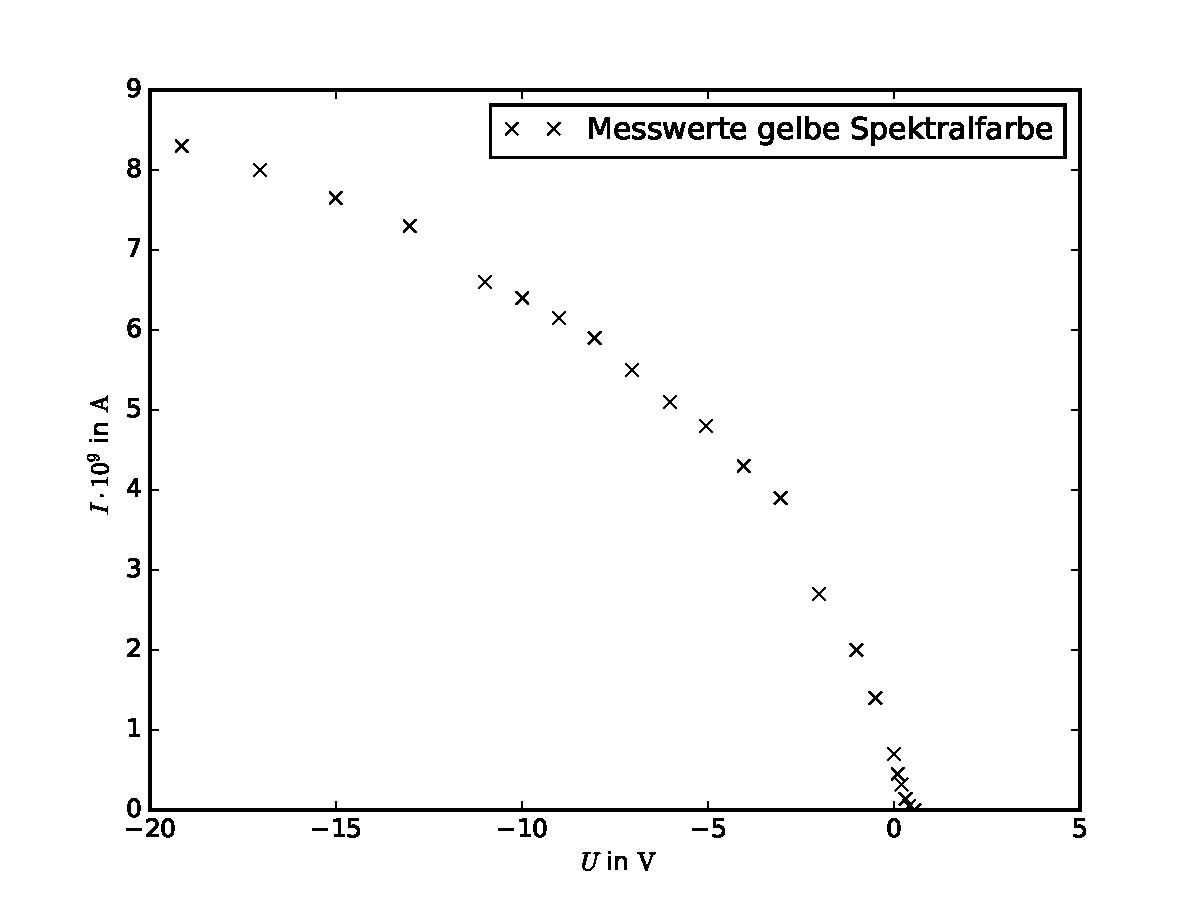
\includegraphics[width = 0.8\textwidth]{Pics/gelbe_Spektrallinie_komplett.pdf}\\[0cm]
    \caption{Gesamtes Messintervall -20 < U < 5 $\su{V}$.}
    \label{fig:Komplett1}
  \end{subfigure}
  \begin{subfigure}{0.8\textwidth}
    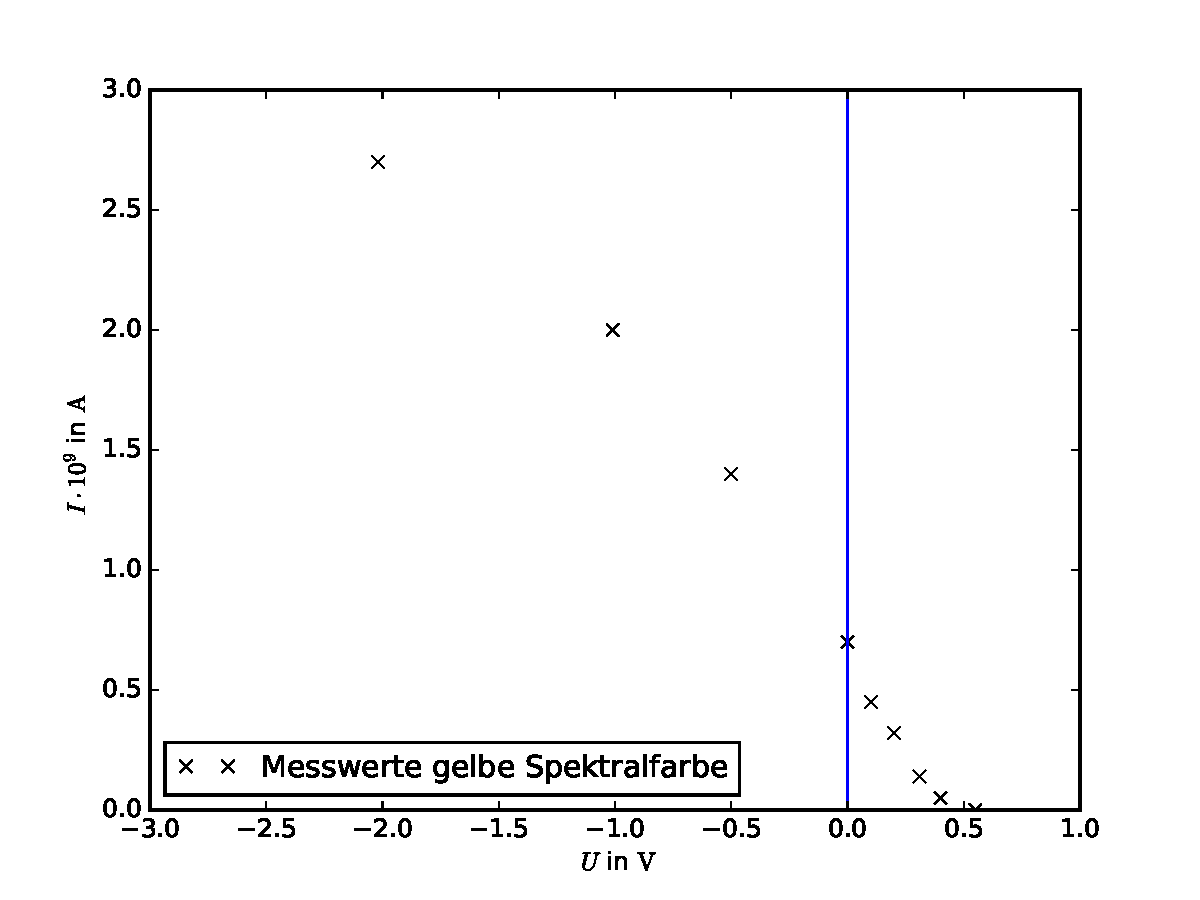
\includegraphics[width = 0.8\textwidth]{Pics/gelbe_Spektrallinie_komplett2.pdf}\\[0cm]
    \caption{Gesamtes Messintervall -3 < U < 1 $\su{V}$.}
    \label{fig:Komplett2}
  \end{subfigure}
  \caption{Gemessene Stromstärke in Abhängigkeit der angelegten Spannung für die
           gelbe Spektralfarbe.}
  \label{fig:GelbKomplett}
\end{figure}

\section{Diskussion}

Bei der Bestimmung der Regressionsparameter im Abschnitt 3.1 traten lediglich
kleine Fehler auf. Bei Abschnitt 3.2 ergab die Regression ziemlich große
Fehler mit einer Regressionsgeraden, die teilweise weit von den Werten entfernt liegt.
Jedoch schneiden die Fehlerbalken größtenteils die Regressionsgerade.
Wird der experimentell bestimmte Wert für $\frac{h}{e\ua{0}}$ mit
dem Literaturwert\cite{Quelle2} verglichen, ist festzustellen, dass eine Abweichung von ca. 44 $\%$
vorliegt.

\begin{align}
  \left( \frac{h}{e\ua{0}} \right)_{\su{lit}}  =  \SI{4.136}{eV}\\
  \left( \frac{h}{e\ua{0}} \right)_{\su{exp}} =  \SI{2.33}{eV}
\end{align}

Für das Auftreten dieses Fehlers sind mehrere Ursachen möglich. Ein große Fehlerquelle
ist dabei vor allem der Aufbau selbst. Das Amperemeter zeigte bei den Messungen
erheblich Schwankungen, weswegen für das gelbe Licht zum Beispiel eine neue Messreihe
angefertigt wurde. Ein Grund hierfür ist auch die verwendete Apparatur. Die Photozelle
wurde mittels einer Schiene auf einem Teilkreisbogen um den Aufbau herumgefahren,
damit die verschiedenen Farbspektren betrachtet werden könen. Jedoch
war die Schiene schief, sodass die Photozelle beim Messen immer wieder leicht
verrutschte und die Intensität nicht konstant gehalten werden konnte. Selbst nach
versuchter Stabilisierung der Schiene ergab sich keine Besserung. Zudem hatte
auch die schwankende Intensität der Hg-Dampflampe noch großen Einfluss auf die
Messwerte.

Eine weitere Fehlerquelle ist vermutlich die Hg-Dampflampe. Bei Betrachtung
der aufgespaltenen Lichtspektren auf einem Schirm war auch deutlich eine rote
Spektralfarbe erkenntlich, welche bei einer Hg-Dampflampe eigentlich nicht vorkommen
sollte. Dieser Effekt beruht vermutlich auf Lufteinschlüsse in der Lampe.

Da der Aufbau wie beschrieben großen Anteil an den auftretenden Fehlern
hat, sind die Abweichungen der bestimmten Werte auf systematische Fehler
zurückzuführen.

Jedoch sind die Grundprinzipien des Photoeffektes bei der verwendeten Apparatur
deutlich geworden, womit das Experiment zur Beobachtung des Photoeffektes
geeignet ist.
